%%%%%%%%%%%%%%%%%%%%%%%%%%%%%%%%%%%%%%%%%%%%%%%%%%%%%%%%%%%%%%%%%
\chapter{FAULT DIAGNOSIS METHODOLOGY}\label{Ch4}
%%%%%%%%%%%%%%%%%%%%%%%%%%%%%%%%%%%%%%%%%%%%%%%%%%%%%%%%%%%%%%%%%
This chapter discusses four different methods for performing fault diagnosis. First of all, different signal processing methods are applied to the 1-phase current signal and compared with machine learning and deep learning methods. In the context of the thesis, two different comparisons are made. The first is to examine the advantages and disadvantages of different feature extraction scenarios and compare them with various metrics, while the second is to examine deep learning methods as an end-to-end solution.
\section{Machine learning analysis}
Machine learning methods need preprocessing for feature extraction, albeit in different ways. These features, which will be utilised for fault detection, directly affect the performance of the classifier. Within the scope of this thesis, three different signal processing for machine learning methods and the calculated features based on this process will be examined. In addition, the responses of the VFD powered motor to different speed and load scenarios are also covered.
\subsection{Time domain statistical analysis}
The first method is to extract the statistical properties of the current data in the time domain and to diagnose faults with machine learning techniques over them. Statistical features such as kurtosis, skewness, mean, RMS, standard deviation and median are extracted in the Knime to be used as features to predict whether the motor is healthy or faulty. 

\begin{landscape}
	\thispagestyle{empty} % Remove the bottom page numbering
%	\begin{changemargin}{-0.4mm}{0mm}{0mm} %Set all the margins to zero - SBÖ
		%\thispagestyle{lscape}

		\vspace*{20mm}
		\begin{figure*}[ht]
			\centering
			%\begin{tabular}{@{}cc@{}}
				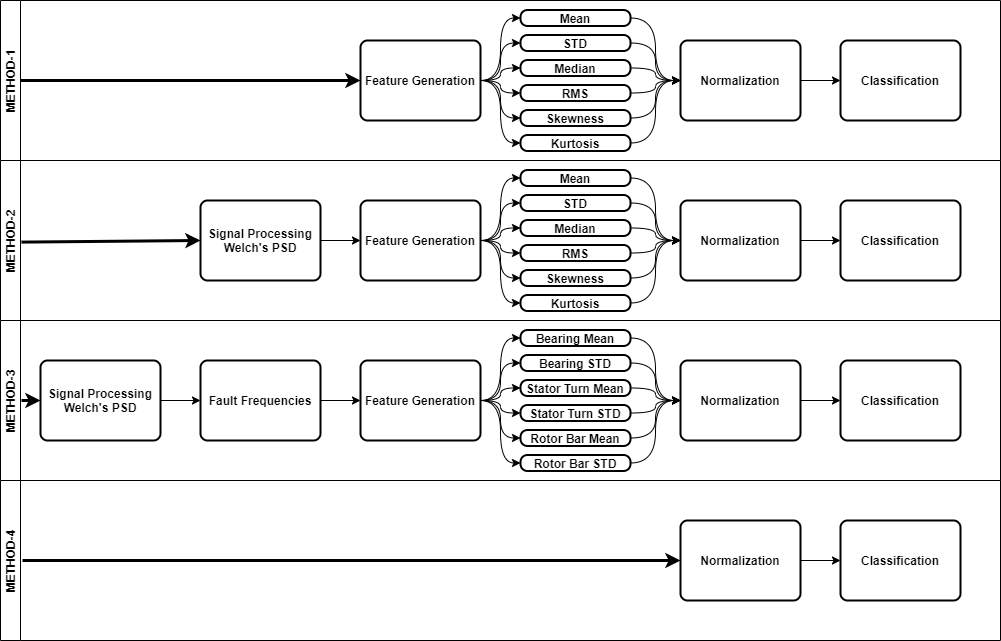
\includegraphics[scale=.45,keepaspectratio=true]{./fig/methods.png} %&
				%
\includegraphics[width=50mm]{./fig/sekil3}
			%\end{tabular}                                       
			\caption{Flowcharts of the methods presented in this thesis.}
			\label{methods}
		\end{figure*}
	   
% % Set the page number on the left side for even numbered pages
% 		\begin{tikzpicture}[remember picture, overlay]
% 		\node[xshift=-25mm+148.5mm, yshift=-1mm-15mm, rotate=180] (number) at (current page text area.east) {\thepage};
% 		\end{tikzpicture}
		
% Set the page number on the right side for even numbered pages as well
		\begin{tikzpicture}[remember picture, overlay]
		 \node[xshift=-25mm+148.5mm, yshift=17mm-210mm] (number) at (current page text area.east) {\thepage};
		\end{tikzpicture}
		
%	\end{changemargin}
\end{landscape}

% All the figures and also odd page figures normally face inside the thesis, however the rule requires figures always face to the right. - SBÖ
% Figures on landscape pages has to be centered and facing to the right (ITU) - SBÖ
% \begin{landscape}
% 	\thispagestyle{empty} %Remove the bottom page numbering
% %	\begin{changemargin}{-0.4mm}{0mm}{0mm} %Set all the margins to zero - SBÖ
% 	%\thispagestyle{lscape}
% 	\vspace*{5mm}
% 	\begin{figure*}
% 		\centering
% 		%\begin{tabular}{@{}cc@{}}
% 		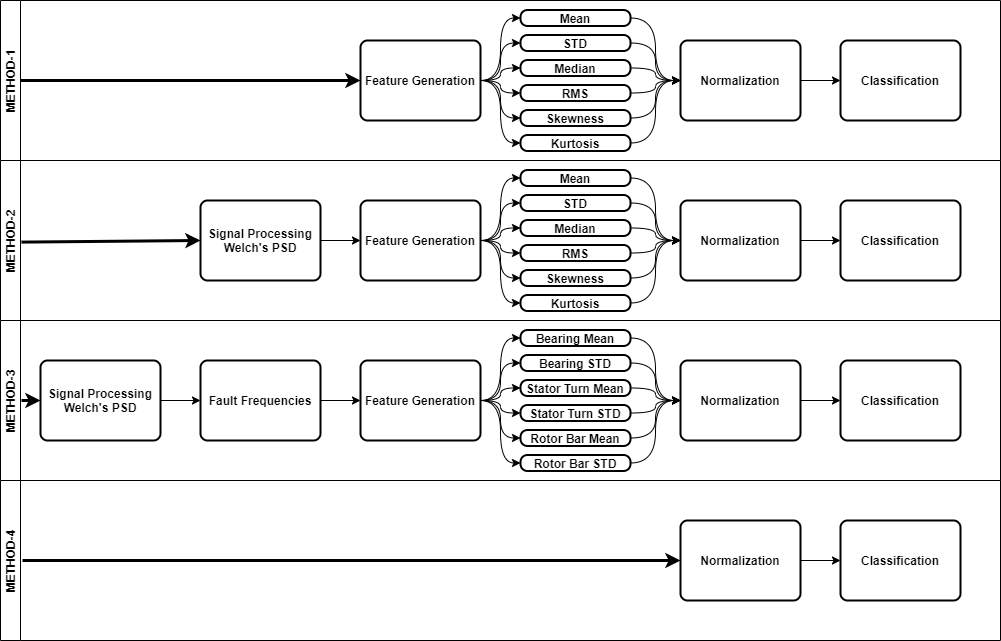
\includegraphics[scale=.45,keepaspectratio=true]{./fig/methods.png} %&
% 		%
\includegraphics[width=50mm]{./fig/sekil3}
% 		%\end{tabular}                                       
% 		\caption{Flowcharts of the methods presented in this thesis.}
% 		\label{methods}
% 	\end{figure*}
	
% % Set the page number on the right side for odd numbered pages
%       \begin{tikzpicture}[remember picture, overlay]
% 		\node[xshift=-25mm+148.5mm, yshift=17mm-210mm+15mm] (number) at (current page text area.east) {\thepage};
% 	  \end{tikzpicture}
	  
% %\end{changemargin}
% \end{landscape}

\begin{figure}[h]
	\centering
	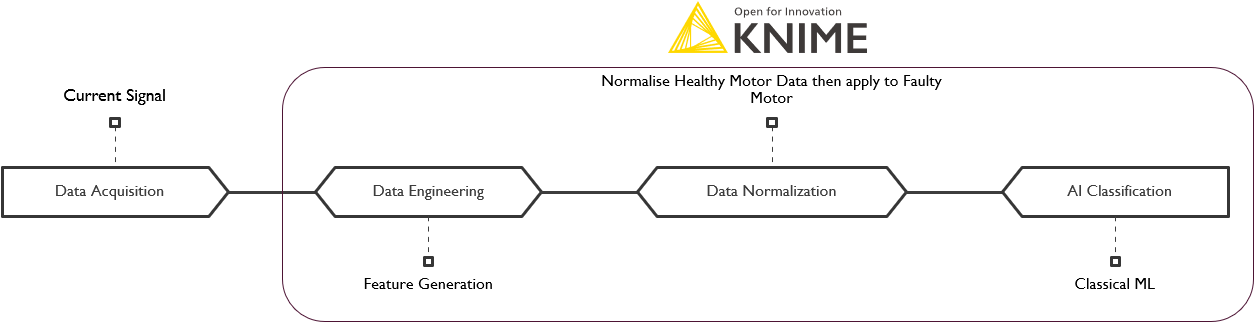
\includegraphics[width=400pt,keepaspectratio=true]{./fig/method1.PNG}
	% sekil3.eps: 0x0 pixel, 300dpi, 0.00x0.00 cm, bb=14 14 1155 740
	\caption{Diagram of time-domain statistical analysis method.}	
	\label{method1}
\end{figure}

In order to examine the distributions of these features in different classes, t-SNE, a manifold learning technique that reduces high-dimensional data to two or three dimensions, was used \cite{van2008visualizing}. It is widely preferred because it can capture nonlinear structures by exploiting local relationships between data points. It is employed to reduce the 6-dimensional feature space to 3 dimensions. It seems that a short-circuit fault between the stator windings and bearing fault can be differentiated from the healthy condition, while a 1-bar broken rotor fault is relatively more difficult to differentiate. This situation can be understood as it does not change the motor behaviour for 1-bar broken rotor failure, but when classification is made with machine learning methods, it is seen that there are algorithms with high performance.

\begin{figure}[h]
	\centering
	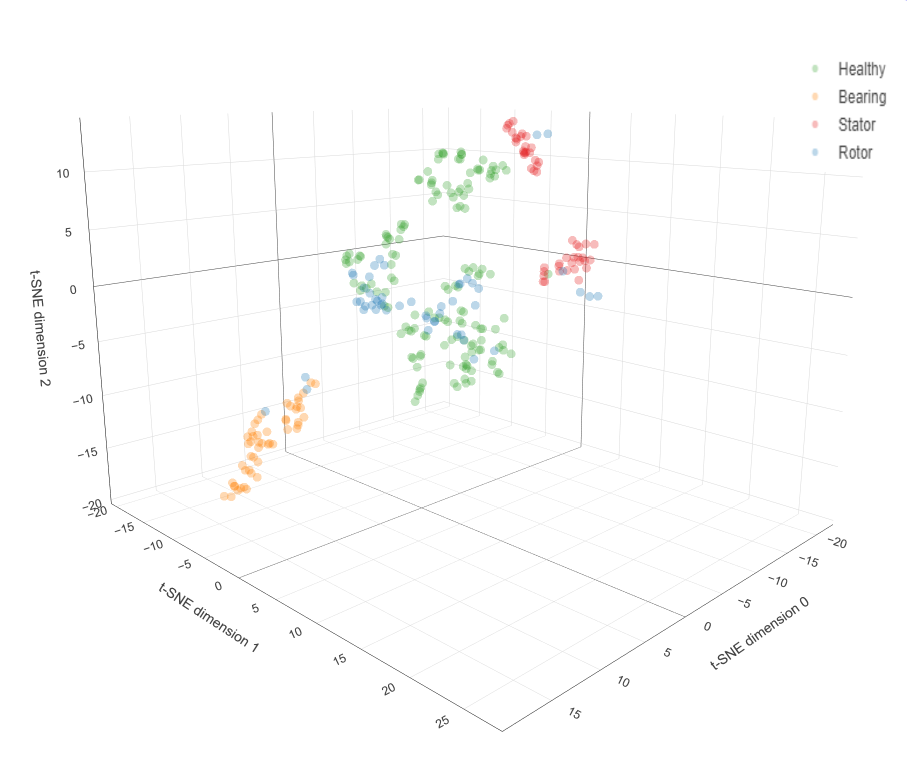
\includegraphics[width=250pt,keepaspectratio=true]{./fig/sne_current.PNG}
	% sekil3.eps: 0x0 pixel, 300dpi, 0.00x0.00 cm, bb=14 14 1155 740
	\caption{t-SNE plot of time-domain statistical features.}	
	\label{snec}
\end{figure}
\pagebreak
\subsection{Frequency domain statistical analysis}

As a second method, by applying Welch's PSD estimation to the current signal, analysis became possible in the frequency domain. After the statistical properties of the amplitudes in the frequency domain were extracted, classification algorithms were applied. As in the first method, statistical properties such as kurtosis, skewness, mean, RMS, standard deviation and median are extracted in the Knime for cases where the motor is healthy or faulty.

\begin{figure}[h]
	\centering
	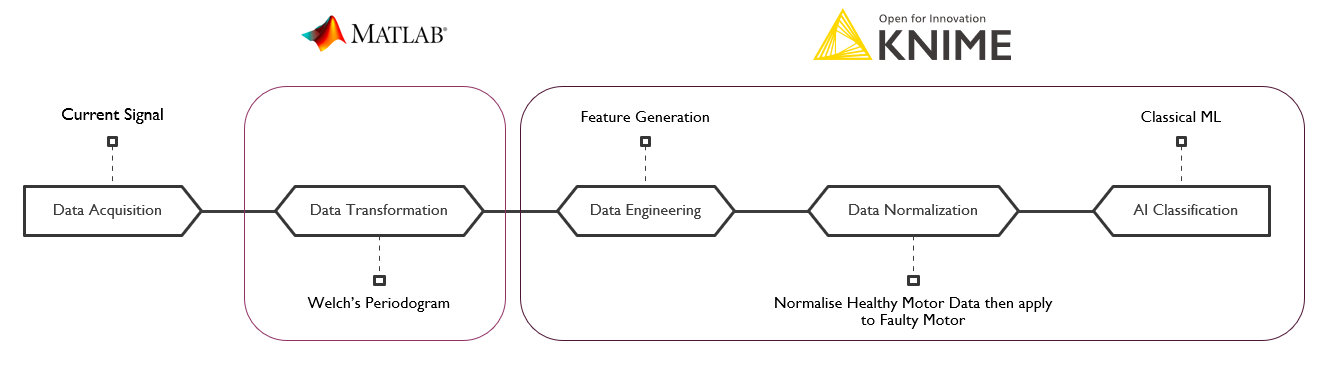
\includegraphics[width=400pt,keepaspectratio=true]{./fig/method2.PNG}
	% sekil3.eps: 0x0 pixel, 300dpi, 0.00x0.00 cm, bb=14 14 1155 740
	\caption{Diagram of frequency domain statistical analysis method.}	
	\label{method2}
\end{figure}

As can be seen from the t-SNE plot, a short-circuit fault between the stator windings and a bearing fault can be better differentiated from the healthy condition than the first method, while 1 bar-broken rotor fault is still relatively more difficult to distinguish. According to the classification performance results, it is seen that a high rate of success can still be achieved.

\begin{figure}[h]
	\centering
	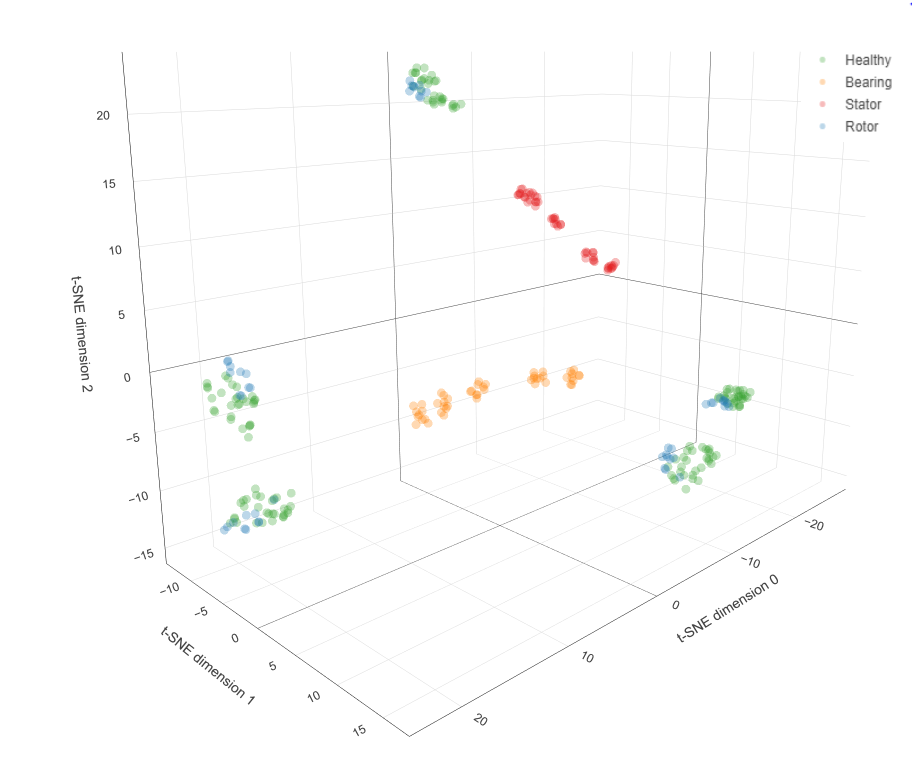
\includegraphics[width=250pt,keepaspectratio=true]{./fig/sne_psd.PNG}
	% sekil3.eps: 0x0 pixel, 300dpi, 0.00x0.00 cm, bb=14 14 1155 740
	\caption{t-SNE plot of frequency domain statistical features.}	
	\label{snep}
\end{figure}
\pagebreak
\subsection{Statistical analysis on characteristic frequencies}

As a third method, by applying Welch's PSD estimate to the current signal, analysis in the frequency domain became possible. Specific fault frequencies in the frequency domain were calculated, then the corresponding amplitudes were calculated. By applying statistical measures such as mean and standard deviation to the amplitudes, six features were created for each condition and classification algorithms were applied to these features. In this method, signal processing and feature extraction are computed in MATLAB, followed by classification in Knime.

\begin{figure}[h]
	\centering
	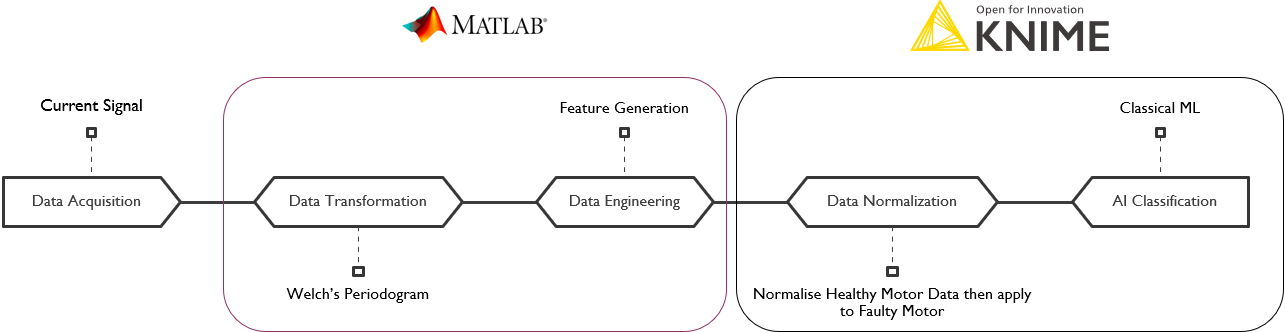
\includegraphics[width=400pt,keepaspectratio=true]{./fig/method3.PNG}
	% sekil3.eps: 0x0 pixel, 300dpi, 0.00x0.00 cm, bb=14 14 1155 740
	\caption{Diagram of statistical analysis of characteristic frequencies method.}	
	\label{method3}
\end{figure}

Condition monitoring and fault diagnosis researches for induction motors have been going on for many years and accordingly, there is a wide knowledge accumulation. Studies in the frequency domain have shown that fault conditions will have certain signs in the frequency spectrum. In this study, using the characteristic frequency equations for bearing, stator and rotor faults given in the literature review section (equations \ref{bearingfault}, \ref{statorfault} and \ref{rotorfault}), it has been calculated up to certain harmonics, and then the mean and standard deviation of the amplitudes corresponding to the frequencies obtained for each fault type are calculated and statistical features are formed.

As can be seen from the t-SNE plot, all faults can be better distinguished from the healthy state than the first and second method. According to the classification performance results, the third method outperforms the other two methods in almost every metric and every classifier.

\begin{figure}[h]
	\centering
	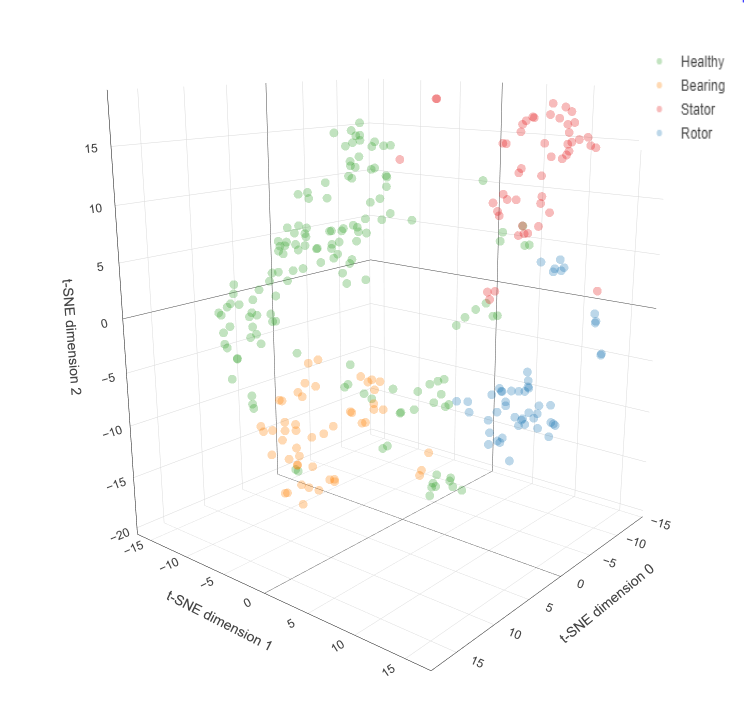
\includegraphics[width=250pt,keepaspectratio=true]{./fig/sne_mcsa.PNG}
	% sekil3.eps: 0x0 pixel, 300dpi, 0.00x0.00 cm, bb=14 14 1155 740
	\caption{t-SNE plot of characteristic frequencies statistics.}	
	\label{snem}
\end{figure}

\subsection{Discussion}

Due to their operating principles, machine learning methods are dependent on data engineering. Features revealed as a result of data engineering can better capture the fault characteristic. As can be seen from Table \ref{compare}, statistical approaches generally yield good results. Another advantage of statistical features is that they can be used in prognostic studies by observing their changes over time. 

Although the statistical study (M1) in the time domain gives good results compared to its simplicity and computational load, it is more vulnerable to external influences. It is useful to approach it carefully, as it is prone to give false results under distorting influences.

PSD estimation with Welch's method is more resistant to disruptive effects due to its properties. While the higher computational load is a disadvantage, it has the potential to show effects that cannot be seen in the time domain. For this reason, it is also used especially in industrial standards. Considering the performance metrics, although the second method (M2) gives close results with the study in the time domain, it can be preferred because it is resistant to external effects.

The characteristic effects of faults on motor current have been known to academic and industrial researchers for a long time. The disadvantage of this method is that it gives good results only under nominal load and speed conditions. However, as revealed in this study, it can be said that it is both a high-performance and robust method by statistically examining the amplitudes at characteristic frequencies (M3) under different speed and load conditions. As Table \ref{compare} exhibits, it outperforms for each performance metric and each classifier compared to other methods.

\begin{landscape}
	\thispagestyle{empty}
%	\vspace*{-6mm}
%	\begin{changemargin}{0.4mm}{0mm}{0mm} %Set all the margins to zero - SBÖ
	\begin{table*}[htb!]
		{\setlength{\tabcolsep}{14pt}
			%\hspace*{5mm}
			%\vspace*{-6mm}
			\caption{Performance metrics for methods and classifiers with 5-fold cross-validation.}
			\begin{center}
				\vspace{-6mm}
				\begin{tabular}{l|lll|lll}
					\hline
					\multicolumn{1}{c}{} & \multicolumn{3}{c}{\begin{tabular}[c]{@{}c@{}}AUC\\      (Mean ± STD)\end{tabular}} & \multicolumn{3}{c}{\begin{tabular}[c]{@{}c@{}}Cohen's Kappa\\      (Mean ± STD)\end{tabular}} \\
					& \multicolumn{1}{c}{M1} & \multicolumn{1}{c}{M2} & \multicolumn{1}{c}{M3} & \multicolumn{1}{c}{M1} & \multicolumn{1}{c}{M2} & \multicolumn{1}{c}{M3} \\
					\hline\\
				   MLP & 0.976 (±0.017) & 0.976 (±0.032) & 0.988 (±0.019) & 0.915 (±0.069) & 0.833 (±0.064) & 0.93 (±0.082) \\
				   SVM & 0.954 (±0.029) & 0.946 (±0.039) & 0.988 (±0.016) & 0.777 (±0.081) & 0.809 (±0.044) & 0.92 (±0.05) \\
				   Random Forest & 0.995 (±0.004) & 0.967 (±0.032) & 0.997 (±0.003) & 0.925 (±0.047) & 0.897 (±0.072) & 0.93 (±0.049) \\
				   XGBoost & 0.986 (±0.014) & 0.953 (±0.022) & 0.992 (±0.007) & 0.871 (±0.059) & 0.847 (±0.079) & 0.914 (±0.046) \\
				   Naive Bayes & 0.948 (±0.019) & 0.884 (±0.027) & 0.989 (±0.004) & 0.792 (±0.052) & 0.662 (±0.146) & 0.876 (±0.049) \\
				   kNN & 0.982 (±0.015) & 0.979 (±0.024) & 0.991 (±0.014) & 0.883 (±0.04) & 0.894 (±0.035) & 0.944 (±0.043) \\ \hline\\
				   


				   & \multicolumn{3}{c}{\begin{tabular}[c]{@{}c@{}}Macro F-measure\\      (Mean ± STD)\end{tabular}} & \multicolumn{3}{c}{\begin{tabular}[c]{@{}c@{}}Accuracy\\      (Mean ± STD)\end{tabular}} \\
				   & \multicolumn{1}{c}{M1} & \multicolumn{1}{c}{M2} & \multicolumn{1}{c}{M3} & \multicolumn{1}{c}{M1} & \multicolumn{1}{c}{M2} & \multicolumn{1}{c}{M3} \\
					\hline
				   MLP & 0.934 (±0.052) & 0.882 (±0.049) & 0.952 (±0.053) & 0.943 (±0.047) & 0.89 (±0.042) & 0.953 (±0.055) \\
				   SVM & 0.908 (±0.054) & 0.856 (±0.029) & 0.947 (±0.033) & 0.86 (±0.048) & 0.877 (±0.03) & 0.947 (±0.033) \\
				   Random Forest & 0.938 (±0.036) & 0.922 (±0.061) & 0.948 (±0.039) & 0.95 (±0.031) & 0.933 (±0.046) & 0.953 (±0.032) \\
				   XGBoost & 0.899 (±0.045) & 0.893 (±0.052) & 0.938 (±0.034) & 0.913 (±0.04) & 0.897 (±0.058) & 0.943 (±0.03) \\
				   Naive Bayes & 0.832 (±0.04) & 0.893 (±0.132) & 0.915 (±0.04) & 0.867 (±0.031) & 0.777 (±0.127) & 0.917 (±0.033) \\
				   kNN & 0.907 (±0.024) & 0.925 (±0.029) & 0.962 (±0.029) & 0.923 (±0.025) & 0.93 (±0.022) & 0.963 (±0.027)\\ \hline 
				\vspace{6mm}
       

					
			\end{tabular}
			\
			\end{center}
			\begin{center}
				\label{compare}
			\end{center}
		}
	\end{table*}
% Set the page number on the right side for odd numbered pages
		\begin{tikzpicture}[remember picture,overlay]
		\node[xshift=-10mm+148.5mm, yshift=2mm-210mm+30mm] (number) at (current page text area.east) {\thepage};
		\end{tikzpicture}
%   \end{changemargin}
\end{landscape}

\section{Deep learning analysis}

In the study, the Tensorflow library was used to develop deep learning models and the Keras interface, which is a software library working on Tensorflow for artificial neural networks, was used in the Knime Data Analytics tool.

\begin{figure}[h]
	\centering
	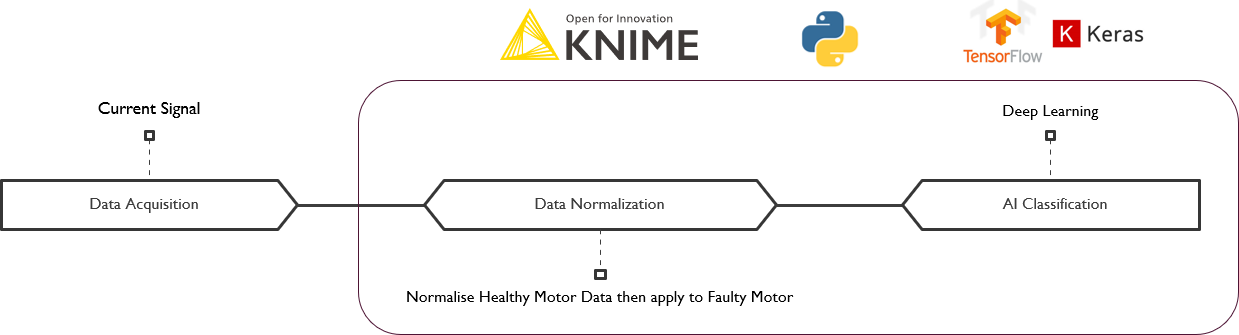
\includegraphics[width=400pt,keepaspectratio=true]{./fig/method4.PNG}
	% sekil3.eps: 0x0 pixel, 300dpi, 0.00x0.00 cm, bb=14 14 1155 740
	\caption{Diagram of deep learning analysis.}	
	\label{method4}
\end{figure}

Since machine learning methods require complex signal processing to extract the characteristics of the given data, the interest in the structures that will work end-to-end between the collected data and the decision output has increased in the industry. Deep learning methods can respond to this interest by not requiring any preprocessing. However, as a downside, large amounts of data are needed to train deep learning methods. In virtue of long-term data collection is not possible in the laboratory environment, the data set was divided into 0.2 seconds segments using the sliding window method with no-overlapping as in \cite{shenfield2020novel}. Original data length in time was 10 seconds, to ensure capturing fault characteristics equation \ref{data} re-calculated and at least 40 times fault impacts captured. Each augmented segments were all assigned the same label as the original input sequence.

\begin{figure}[h]
	\centering
	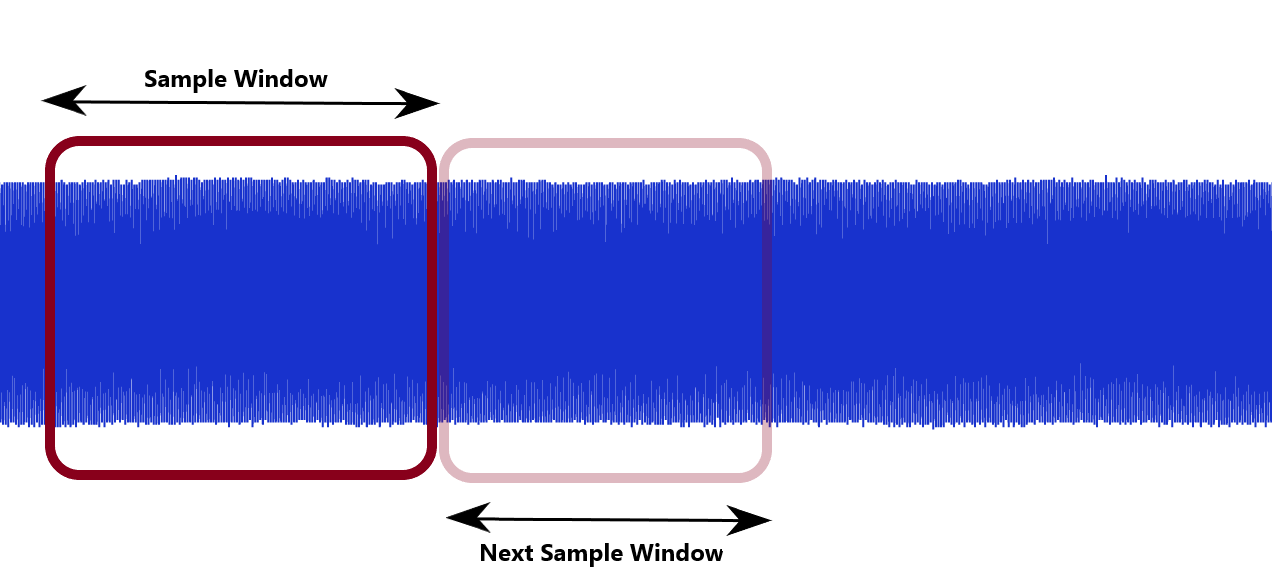
\includegraphics[width=300pt,keepaspectratio=true]{./fig/data.png}
	% sekil3.eps: 0x0 pixel, 300dpi, 0.00x0.00 cm, bb=14 14 1155 740
	\caption{Sliding window data augmentation.}	
	\label{dataslide}
\end{figure}

The augmented dataset was used in the training of two different deep learning methods: Convolutional Neural Networks and LSTM Networks. Although CNN originated and mostly applied on 2-dimensional problems mainly in computer vision studies, 1-D CNN successfully applied on time series signals such as vibration, sound and current fault diagnosis of induction motors \cite{eren2017bearing,eren2019generic,qiao2020deep,skowron2020convolutional}.

An improved 1D-CNN structure for bearing fault diagnosis presented in \cite{chen2021improved}, in this thesis study, structure improved further to the extended diagnosis of the stator winding short-circuit and broken rotor bar faults also.

\begin{table*}[h]
	{\setlength{\tabcolsep}{12pt}
 		\caption{1D- CNN structure.}
 		\begin{center}
 			\vspace{-6mm}
			\begin{tabular}{ccc}
				\hline \\[-2.45ex] \hline \\[-2.1ex]
			\textbf{Type}               & \textbf{Shape}             & \textbf{Specific Setting} \\
				\hline	
			Input              & (1000$\times$ 1)   & 5 kHz-0.2sec             \\				
			Conv1D             & (None, 1000, 128) & 128@16x1, stride =1      \\
			BatchNormalization & (None, 1000, 128) & -                        \\
			MaxPooling1D       & (None, 500, 128)  & pool size 2x1, stride =2 \\
			Dropout            & (None, 500, 128)  & 0.25                     \\
			Conv1D             & (None, 500, 64)   & 64@8x1, stride =1        \\
			BatchNormalization & (None, 500, 64)   & -                        \\
			MaxPooling1D       & (None, 250, 64)   & pool size 2x1, stride =2 \\
			Dropout            & (None, 250, 64)   & 0.25                     \\
			Conv1D             & (None, 250, 32)   & 32@4x1, stride =1        \\
			BatchNormalization & (None, 250, 32)   & -                        \\
			MaxPooling1D       & (None, 125, 32)   & pool size 2x1, stride =2 \\
			Dropout            & (None, 125, 32)   & 0.1                      \\
			Conv1D             & (None, 125, 16)   & 16@4x1, stride =1        \\
			BatchNormalization & (None, 125, 16)   & -                        \\
			MaxPooling1D       & (None, 62, 16)    & pool size 2x1, stride =2 \\
			Dropout            & (None, 62, 16)    & 0.1                      \\
			Conv1D             & (None, 62, 8)     & 8@4x1, stride =1         \\
			BatchNormalization & (None, 62, 8)     & -                        \\
			MaxPooling1D       & (None, 31, 8)     & pool size 2x1, stride =2 \\
			Dropout            & (None, 31, 8)     & 0.25                     \\
			Flatten            & (None, 248)       &                          \\
			Dense              & (None, 4)         &                         \\				
				\hline
			\end{tabular}
			\vspace{-6mm}
		\end{center}}
		\label{cnn}
\end{table*}

RNN is preferred in condition monitoring diagnostic applications because of its ability to work with sequential data. Since RNNs learn by backpropagation in time during a supervised learning process, problems with gradients during training can result in the increased error in time steps or distortion of prior knowledge \cite{enshaei2019application}. In order to overcome this disadvantage, LSTMs have been developed to capture existing dependencies in time series data. Many studies have been carried out with LSTM networks for fault detection and the effectiveness of the structure has been demonstrated \cite{bai2021long,he2021fpga,khan2018review,sabir2019lstm}.

\begin{table*}[h]
	{\setlength{\tabcolsep}{12pt}
 		\caption{LSTM structure.}
 		\begin{center}
 			\vspace{-6mm}
			\begin{tabular}{ccc}
				\hline \\[-2.45ex] \hline \\[-2.1ex]
			\textbf{Type}               & \textbf{Shape}             & \textbf{Specific Setting} \\
				\hline	
			Input              & (1000$\times$ 1)   & 5 kHz-0.2sec             \\				
			LSTM               & (None, 1000, 8)  & \begin{tabular}[c]{@{}c@{}}units = 8\\ activation =  'tanh'\\ recurrent activation = 'sigmoid'\end{tabular}  \\
			BatchNormalization & (None, 1000, 8)  & -                                                                                                            \\
			Dropout            & (None, 1000, 8)  & 0.5                                                                                                          \\
			LSTM               & (None, 1000, 16) & \begin{tabular}[c]{@{}c@{}}units = 16\\ activation =  'tanh'\\ recurrent activation = 'sigmoid'\end{tabular} \\
			BatchNormalization & (None, 1000, 16) & -                                                                                                            \\
			Dropout            & (None, 1000, 16) & 0.4                                                                                                          \\
			LSTM               & (None, 1000, 16) & \begin{tabular}[c]{@{}c@{}}units = 16\\ activation =  'tanh'\\ recurrent activation = 'sigmoid'\end{tabular} \\
			BatchNormalization & (None, 1000, 16) & -                                                                                                            \\
			Dropout            & (None, 1000, 16) & 0.4                                                                                                          \\
			Flatten            & (None, 16000)    &                                                                                                              \\
			Dense              & (None, 4)        &           \\                                                                                                  				
				\hline
			\end{tabular}
			\vspace{-6mm}
		\end{center}}
		\label{lstm}
\end{table*}

Detailed representations of 1D-CNN and LSTM structures are given in the appendix. 

As given in Table \ref{deepl}, both deep learning methods provide impressive results in the diagnostics of faults. Comparing the two methods, 1D-CNN outperforms LSTM in all metrics, while LSTM is simpler and straightforward in structure. However, the time required to train both models is the same.

\begin{table*}[h]
	{\setlength{\tabcolsep}{12pt}
 		\caption{Performance metrics for deep learning architectures.}
 		\begin{center}
 			\vspace{-6mm}
			\begin{tabular}{c|cccc}
				\hline \\[-2.45ex] \hline \\[-2.1ex]
				& AUC   & Cohen's Kappa & Macro F-measure & Accuracy \\

				\hline

			1D-CNN & 0.955 & 0.922         & 0.944           & 0.947    \\

			LSTM   & 0.936 & 0.87          & 0.904           & 0.912   \\
				\hline
			\end{tabular}
			\vspace{-6mm}
		\end{center}
		\label{deepl}}
\end{table*}

\begin{figure}[h]
	\begin{subfigure}[b]{.5\linewidth}
		\centering
		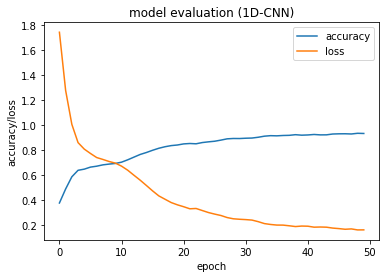
\includegraphics[scale=.5]{./fig/cnn_accloss.png}
		\firstsubcaption{Training performance of 1D-CNN model.}\label{tracnn}
	\end{subfigure}
	\begin{subfigure}[b]{.5\linewidth}
		\centering
		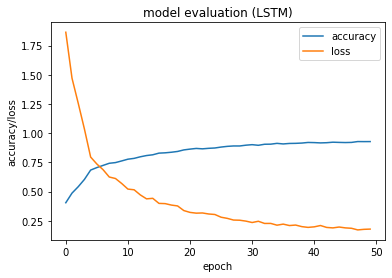
\includegraphics[scale=.5]{./fig/lstmaccloss.png}
		\nextsubcaption{Training performance of LSTM model.}\label{tralstm}
	\end{subfigure}
	%\caption{A figure}\label{Figure2.2} % If no need a caption for main figure comment it out 
\end{figure}
%Figure letter: \subref{Figure2.2a}

\section{Discussion}

Machine learning methods can give better results than deep learning methods in relatively small datasets such as datasets obtained in experimental studies. As shown in Table \ref{compare}, machine learning methods give successful results. It has been demonstrated that machine learning algorithms show high performance, especially when the features made with statistical calculations at characteristic failure frequencies specified as the third method are used. However, it is obvious that it requires complex calculations and developer-based competence to achieve high performance.

As presented in Table \ref{deepl}, although deep learning methods are trained with much less data samples than machine learning methods, they gave very close results with machine learning methods trained with features extracted by the third method. In addition, it is another important issue that it provides such high performance without the need for any data preprocessing.

It can be said that the performance of deep learning methods will increase even more with the amount of data increasing with a high acceleration in industrial applications. Pre-trained deep learning models can also be useful in embedded systems with constrained resources. Especially, a deep learning-based condition monitoring and fault recognition application that will be integrated into motor drivers has great potential.